\documentclass{article}
\usepackage[utf8]{inputenc}

\usepackage[a4paper, total={6in, 9in}]{geometry}
\usepackage{graphicx}
\usepackage{mathtools}
\graphicspath{{./figures/}}
\usepackage{rotating}
\usepackage[section]{placeins}
\DeclareGraphicsExtensions{.pdf,.jpeg,.png}
\DeclarePairedDelimiter\set\{\}

\title{\LARGE \bf System Architecture and Specifications}
\author{O.~Can~G\"{o}r\"{u}r$^{*}$, Jacob Seibert, Malte Siemers, Marc Schmidt}
\date{}

\begin{document}
\maketitle

\section{System Architecture}

A visualisation of our system architecture is provided in Figure \ref{arch} below. It shows the connections between the different system components that will be implemented as ROS nodes. The data show is represented by the arrows. Since the agents are the part of the system doing the most extensive computation work, their
operations are presented there too.

The same architecture is visualized as ROS node graph using the ros package $rqt_graph$ in Figure \ref{rqt}.

\section{System Specification}
\subsection{Warehouse Management}
The Warehouse Management has access to all the data, that is required to obtain a certain model of a warehouse. This static data is used to describe the physics of the system as well as to configure the different components of it as required.

The Warehouse Management is responsible for getting the whole
system started with the predefined configurations and to stop the incoming of new tasks to shutdown the system if that is demanded.

\begin{figure}[t!]
	\centering
	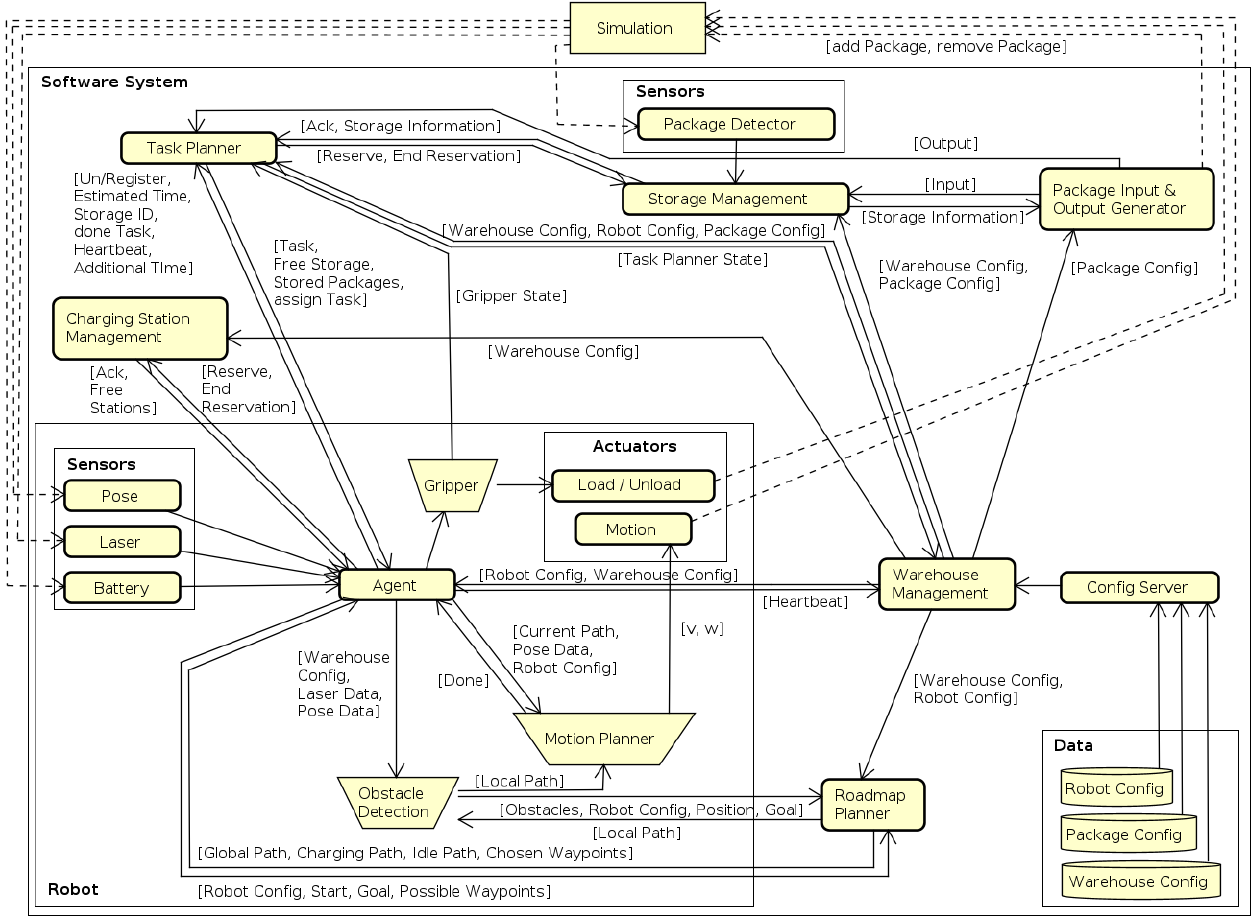
\includegraphics[scale=0.3,natwidth=1189,natheight=915]{architecture}
	\caption{The overall System Architecture}
	\label{arch}
\end{figure}

\begin{sidewaysfigure}[ht]
	\centering
	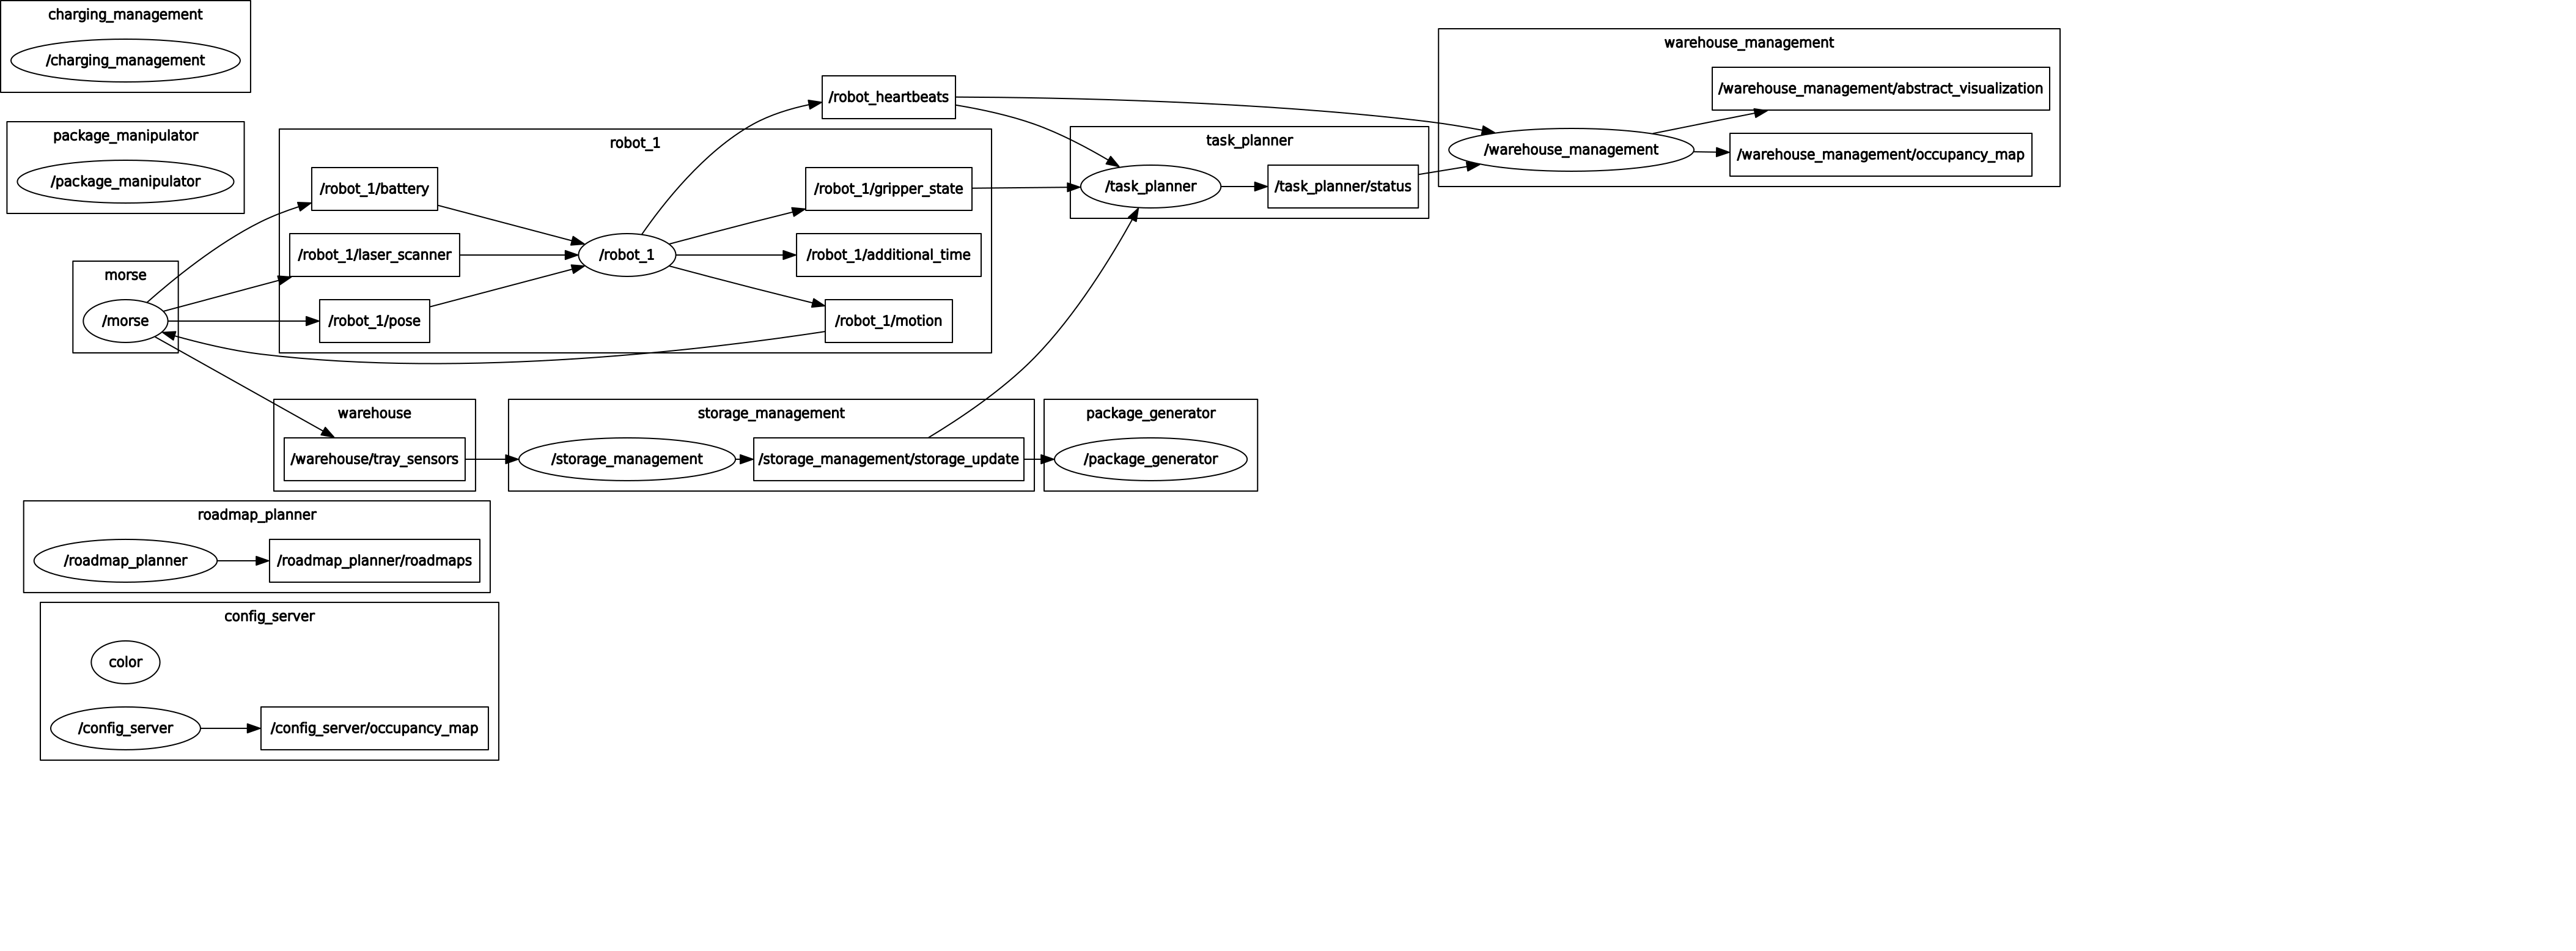
\includegraphics[scale=0.25,natwidth=4214,natheight=1555]{rosgraph}
	\caption{ROS Node graph, $rqt_graph$, of the integrated system}
	\label{rqt}
\end{sidewaysfigure}

\begin{enumerate}
  \item[\textit{i)}] Data 
  \begin{itemize}
    \item Map: one map per simulation only
    \begin{itemize}
      \item geometry of the environment
      \item locations of input, output \& storage
      \item charging zones: rectangle locations in the x-y coordinate plane with preset charging rates
      \item start / rest locations for robots: robots rest there if they are idle
    \end{itemize}
    \item Package Config: contains as many different package configurations as different packages needed
    \begin{itemize}
      \item $Package\_Type$: all packages of a type are considered as equal, so if a package is requested at the output the software system only needs to care about the type of that package
      \item $Package\_Weight$: the weight of the package determines which robots are able to carry that package
      \item $Package\_Geometry$: the geometry of the package determines which robots are able to carry that package
	\end{itemize}
	\item  Robot Config: contains as many robot configurations as different robot types needed
	Since we use only robots with differential drive the robots are capable of turning on spot so that we don't need to set a minimal turning radius in the robot configurations.
	\begin{itemize}	  
		\item $Max\_Speed$: the maximal velocity the robot is able to drive with
		\item $Robot\_Radius$: minimal radius of a circle centered in the middle of the robot, such that the circle covers the robot extent
		\item $Max\_Carry\_Weight$: the maximal weight the robot is able to carry
		\item $Carry\_Geometries$: a list of all the geometries the robot is able to carry
		\item $Discharging\_Rate$: battery discharging rate in percent per second
	\end{itemize}
	\item Charging Config: contains one charging configuration per charging zone
	\begin{itemize}
	   \item $Max\_Number\_Robots$: The maximum number of robots that can be charged simultaneously.
	\end{itemize}
	\item Roadmap: one roadmap per robot configuration
	\begin{itemize}
	   \item is generated while running time by the Roadmap Generator
	   \item a static set of roads the robot is able to drive o
	   \item is represented as a graph: the nodes are associated with the different waypoint positions on the map, the edges specify which waypoints are directly reachable (in a straight line) from a certain waypoint and the edge weights contain the estimated time a robot would take to drive from one of this edge defining nodes to the other.
	\end{itemize}
 	\end{itemize}
 	
  \item[\textit{ii)}] Service Requests
  \begin{itemize}
  	\item Roadmap Generator
  	\begin{itemize}
  		\item generateRoadmap($Map, Robot\_Config$) : Roadmap
  		\begin{itemize}
  			\item at the beginning of the simulation the Warehouse Manager requests the Roadmap Generator to create one Roadmap per robot configuration
			\item Roadmaps are required to start the agents because they contain the data to plan the path for the robot
  		\end{itemize}
  	\end{itemize}
  	\item Package Input \& Output Generator
	\begin{itemize}
		\item start($Package\_Config$) : boolean
		\begin{itemize}
			\item after all other components have been launched, finally the Package Input \& Output Generator has to be started to simulate requests to store or retrieve packages
		\end{itemize}
		\item stop() : boolean
	\end{itemize}
	\item Storage Management
	\begin{itemize}
		\item start($Map, Package\_Config$) : boolean
	\end{itemize}
	\item Task Planner
	\begin{itemize}
		\item start($Map, Robot\_Config, Package\_Config$) : boolean
	\end{itemize}
	\item Agent
	\begin{itemize}
		\item start($Agent\_ID, Map, Robot\_Config, Roadmap$) : boolean
	\end{itemize}
	\item Charging Station Management
	\begin{itemize}
		\item start($Map, Charging\_Config$) : boolean
	\end{itemize}
  \end{itemize}    
\end{enumerate}

\subsection{Roadmap Generator}
The Roadmap Generator offers a service to create roads on a static map with respect to the physical constraints of the vehicles that are about to use this roads.
\begin{enumerate}
	\item[\textit{i)}] Service Offers
	\begin{itemize}
		\item generateRoadmap(Map, $Robot\_Config$) : Roadmap
		\begin{itemize}
			\item generates a Roadmap with respect to the static obstacles the Map contains as well as the $Robot\_Config$ which determines which movement behaviour the specific kind of robot has.
			\item the Map contains important locations the roads have to cover e.g. input / output \& storage locations, charging zones, start / rest locations, . . .
		\end{itemize}
	\end{itemize}
\end{enumerate}

\subsection{Package Input and Output Generator}
The Package Input \& Output Generator simulates a source such that packages arrive at the input for storage in the warehouse as well as it simulates a sink where a specific type of package is demanded at some given output and the system shall provide that package there as soon as possible. The generation of requests shall be random.
\begin{enumerate}
	\item[\textit{i)}] Service Offers
	\begin{itemize}
		\item start($Package\_Config$) : boolean
		\begin{itemize}
			\item hands over the package configurations
			\item starts to simulate package sources as well as package sinks
			\item requests storage information from the Storage Management
		\end{itemize}
		\item stop() : boolean
		\begin{itemize}
			\item stops to create new packages at the inputs as well as it stops to demand stored packages at the outputs (delivery points for logistics).
		\end{itemize}
	\end{itemize}
	\item[\textit{ii)}] Service Requests
	\begin{itemize}
		\item Storage Management
		\begin{itemize}
			\item getStorageInformation() : $Storage\_Information$
			\begin{itemize}
				\item directly after being started, the Package Input \& Output Generator asks for the storage informations, to get the required informations for generating inputs \& outputs.
			\end{itemize}
			\item newInput($Input\_ID, Package\_ID, Package\_Type$) : boolean
			\item newOutput($Output\_ID, Package\_Type$) : boolean
		\end{itemize}
	\end{itemize}
	\item[\textit{iii)}] Topics Subscribed
	\begin{itemize}
		\item Storage Management
		\begin{itemize}
			\item Storage Information
			\begin{itemize}
				\item used to stay up to date with the storage informations
				\item informations are published when the state of the warehouse storage changed
				\item required to know where to add input and which output to request
			\end{itemize}
		\end{itemize}
	\end{itemize}
\end{enumerate}

\subsection{Storage Management}
The Storage Management has an overview of the overall storage of the warehouse and provides those information, performs administrative tasks like reservation of storage and informs the Taskplanner about incoming Tasks. Furthermore the Storage Management is able to detect if a package is stored at a certain
storage location so that loading as well as unloading packages is doublechecked.

\begin{enumerate}
	\item[\textit{i)}] Service Offers
	\begin{itemize}
		\item start($Map, Package\_Config$) : boolean
		\begin{itemize}
			\item  hands over the map as well as the package configurations.
			\item starts all other services and publishes the storage informations topic.
		\end{itemize}
		\item getStorageInformation() : $Storage\_Information$
		\begin{itemize}
			\item provides the storage informations of the whole warehouse.
			\item useful at start because the storage information topic only publishes if the package detectors
recognized some change.
		\end{itemize}
		\item newInput($Input\_ID, Package\_ID, Package\_Type$) : boolean
		\begin{itemize}
			\item  a new package with a given id and type has been arrived at the input container with the given id.
			\item saves the id and type of the package corresponding to the input container with the given id.
			\item expects the package detection laser to recognize an incoming package at the input with the given id and marks that input as reserved.
		\end{itemize}
		\item newOutput($Output\_ID, Package\_Type$) : boolean
		\begin{itemize}
			\item a package of the given type is demanded at the output container with the given id.
			\item saves the type of the package corresponding to the output container with the given id.
			\item  expects the package detection laser to recognize an incoming package at the output with the given id and marks that output as reserved.
		\end{itemize}
		\item reserveStorage($Storage\_ID$) : boolean
		\begin{itemize}
			\item questions to reserve the storage with the given id.
			\item reserved storage is not marked as free storage.
			\item returns if the storage is reserved.
		\end{itemize}
		\item endReservation($Storage\_ID$) : boolean
		\begin{itemize}
			\item questions to end reservation of the storage with the given id.
			\item the storage is marked as free again.
			\item returns if the reservation has been ended.
		\end{itemize}
	\end{itemize}
	\item[\textit{ii)}] Topics Published
	\begin{itemize}
		\item Storage Information
		Every time a package has been placed into or has been retrieved from a storage container and every time a storage container is reserved or not any longer reserved the Storage Informations are published.
		\begin{itemize}
			\item $Free\_Input$: $Input\_ID$'s of the input containers that are empty
			\item $Free\_Output$: $Output\_ID$'s of the output containers that are empty
			\item $Free\_Storage$: $Storage\_ID$'s of the storage containers that are empty
			\item $Stored\_Packages$: information about where and which packages are stored in the warehouse e.g. $Storage\_ID, Package\_ID, Package\_Type$,. . .
			\item $Full\_Output$: $Output\_ID$'s of the output containers that are full
		\end{itemize}
	\end{itemize}
	\item[\textit{iii)}] Service Requests
	\begin{itemize}
		\item Task Planner
		\begin{itemize}
			\item storePackage($Input\_ID, Package\_ID, Package\_Type$) : boolean
			\begin{itemize}
				\item after getting the new input request and detecting some package at the corresponding input the task is sent to the planner.
			\end{itemize}
			\item retrievePackage($Output\_ID, Package\_Type$) : boolean
			\begin{itemize}
				\item after getting the new output request and making sure such a package type is stored in the warehouse already the task is sent to the planner.
			\end{itemize}
		\end{itemize}
	\end{itemize}
	\item[\textit{iv)}] Topics Subscribed
	\begin{itemize}
		\item Package Detector Sensor: one per input tray, output tray \& storage containers on the map
		\begin{itemize}
			\item $Package\_Present$
			\begin{itemize}
				\item detects whether a package is present at the container or not.
				\item could be handled by collision detection or laser detection.
			\end{itemize}
		\end{itemize}
	\end{itemize}
\end{enumerate}

\subsection{Task Planner}
The Task Planner receives tasks, decides which kind of robot is capable to fulfill those, requests how much time it would take for the suitable robots to accomplish the task, decides which robot is the most available one and assigns the task to it.

\begin{enumerate}
	\item[\textit{i)}] Service Offers
	\begin{itemize}
		\item start($Robot\_Config, Package\_Config$) : boolean
		\begin{itemize}
			\item hands over the map, the robot configurations and the package configurations.
			\item starts all other services.
		\end{itemize}
		\item storePackage($Input\_ID, Package\_ID, Package\_Type$) : boolean
		\begin{itemize}
			\item a package with the given id and type arrived at the input with the given id and is ready to be stored in the warehouse.
			\item chooses which of the registered robots are capable of fulfilling the task and sends the store request to them.
		\end{itemize}
		\item retrievePackage($Output\_ID, Package\_Type$) : boolean
		\begin{itemize}
			\item  a package with a given type is demanded at the input with the given id.
			\item chooses which of the registered robots are capable of fulfilling the task and sends the retrieve request to them.
		\end{itemize}
		\item register($Agent\_ID$) : boolean
		\begin{itemize}
			\item registers the agent with the given id.
			\item registered agents receive task requests.
		\end{itemize}
		\item unregister($Agent\_ID$) : boolean
		\begin{itemize}
			\item unregisters an agent to avoid receiving task requests.
			\item reserved storage is not marked as free storage.
			\item returns if the storage is reserved.
		\end{itemize}
		\item endReservation($Storage\_ID$) : boolean
		\begin{itemize}
			\item questions to end reservation of the storage with the given id.
			\item will be called if the battery of an Agent is below some minimum and it's not clear if the Charging Station is going to be reached before it's empty.
		\end{itemize}
		\item completedTask($Task\_ID$) : boolean
		\begin{itemize}
			\item called by an agent if the task with the given id has been fulfilled.
			\item when the Storage Management provides the expected Storage Information the task is completed.
		\end{itemize}
	\end{itemize}
	\item[\textit{ii)}] Service Requests
	\begin{itemize}
		\item Agent
		\begin{itemize}
			\item store($Task\_ID, Input\_ID, Free\_Storage$) : $Storage\_ID, Estimated\_Time$
			\item retrieve($Task\_ID, Output\_ID, Stored\_Packages$) : $Storage\_ID, Estimated\_Time$
			\item assignTask($Task\_ID$) : boolean
			\begin{itemize}
				\item choose agent with the lowest estimated time for that task
				\item before calling this tell the Storage Management must have reserved the corresponding storage.
			\end{itemize}
		\end{itemize}
		\item Storage Management
		\begin{itemize}
			\item reserveStorage($Storage\_ID$) : boolean
			\begin{itemize}
				\item requests to reserve storage if an agent asked to do so.
			\end{itemize}
			\item endReservation($Storage\_ID$) : boolean
			\begin{itemize}
				\item requests to end reservation if an agent asked to do so or if the associated task is complete.
			\end{itemize}
		\end{itemize}
	\end{itemize}
	\item[\textit{iii)}] Topics Subscribed
	\begin{itemize}
		\item Storage Management
		\begin{itemize}
			\item Storage Information
			\begin{itemize}
				\item needs storage informations to tell the agents which possibilities they have to store the package at or retrieve the package from.
			\end{itemize}
		\end{itemize}
	\end{itemize}
\end{enumerate}

\subsection{Agent}
The Agents are the executive components of the whole system. They receive requests to calculate how
much time they would require to fulfill a specific task and have to take care of those tasks. Doing this the battery level is considered to include visiting charging zones which should be integrated into the calculation of the duration the task could be fulfilled in. The Agents have access to a pose, laser and battery sensor to get information about their location and their local environment as well as they have access to load / unload and motion actuators to interact with their environment.

\begin{enumerate}
	\item[\textit{i)}] Operations
	\begin{itemize}
		\item detectObstacles($Laser\_Data, Pose\_Data, Map$) : Obstacle
		\begin{itemize}
			\item if the laser data doesn't match the data of the static obstacles on the map the unexpected obstacle is returned
			\item an obstacle consists of a set of points in the x-y coordinate plane
			\item no complex algorithm needed, just match the laser data with the static obstacles
			\item returns NULL if no Obstacle detected
		\end{itemize}
		\item planPathToStorage($Input\_ID, Free\_Storage, Pose\_Data, Roadmap, Battery\_Level$) : $Path, Storage\_ID, Estimated\_Time$)
		\begin{itemize}
			\item calculates the shortest path on the roadmap that is required to store the package at the input with the given id.
			\item considering the battery level it takes the visit of charging stations into account in the computation
			\item chooses one of the empty storage containers to store the package at start point of the path is the destination of the last task in the taskqueue of the robot and the battery level is the estimated battery level at this location 
			\item shortest path finding with dijkstra
		\end{itemize}
		\item planPathToDeliver($Output\_ID, Package\_Type, Stored\_Packages, Pose\_Data, Roadmap$) : $Path, Storage\_ID, Estimated\_Time$)
		\begin{itemize}
			\item calculates the shortest path on the roadmap that is required to deliver a stored package of the given type to the output with the given id.
			\item considering the battery level it takes the visit of charging stations into account in the computation.
			\item chooses one of the containers that contain the given package type to retrieve the package from start point of the path is the destination of the last task in the taskqueue of the robot and the battery level is the estimated battery level at this location.
		\end{itemize}
		\item planTrajectory($Map, Obstacle, Pose\_Data, Current\_Path, Robot\_Config$) : $Path, Estimated\_Time$)
		\begin{itemize}
			\item is triggered when an obstacle is detected. 
			\item calculates the shortest path back to the current path considering the given obstacle, the map and the robot configuration.
			\item may skip some of the waypoints of the current path but may not skip subgoals e.g. storage
location to load / unload a package
			\item start point of the returned path is the current location of the robot and the destination point of the returned path is some point of the current path
			\item use the D* algorithm here
		\end{itemize}
		\item planMotion($Current\_Path, Pose\_Data, Robot\_Configuration$) : boolean
		\begin{itemize}
			\item adjusts the parameters of the motion actuator to drive along the given current path and takes into account the current pose data as well as the robot configuration.
			\item tells motion actuator which linear and angular velocity to set
			\item returns true if already at destination
		\end{itemize}
	\end{itemize}
	\item[\textit{ii)}] Service Offers
	\begin{itemize}
		\item start($Agent\_ID, Map, Robot\_Config, Roadmap$) : boolean
		\begin{itemize}
			\item hands over the agent id, the map, the robot configuration and the roadmap associated to the robot configuration.
			\item starts all other services.
			\item calls the register service at the task planner.
		\end{itemize}
		\item store($Task\_ID, Input\_ID, Free\_Storage$) : $Storage\_ID, Estimated\_Time$
		\begin{itemize}
			\item request to plan the storing of a package which is located at the input with the given id.
			\item returns the estimated time for this task in addition to the time for completing all other tasks in the taskqueue and returns the id of the storage the package should be stored at.
			\item calls planPathToDeliver with the associated parameters.
			\item saves task as well as calculation results temporarily.
		\end{itemize}
		\item assignTask($Task\_ID$) : boolean
		\begin{itemize}
			\item assigns the task with the given id to this agent
			\item the task is placed at the last position of the taskqueue of the agent.
			\item we know which task to fulfill because we saved it temporarily before.
			\item calls reserveChargingZone
		\end{itemize}
	\end{itemize}
	\item[\textit{iii)}] Service Requests
	\begin{itemize}
		\item Charging Station Management
		\begin{itemize}
			\item reserveChargingZone($Agent\_ID, ChargingZone\_ID$) : boolean
			\begin{itemize}
				\item will be called after a task is assigned and it requires charging to fulfill the task
			\end{itemize}
			\item chargeRequest($Agent\_ID, ChargingZone\_ID$) : boolean
			\begin{itemize}
				\item triggered a short time before the robot wants to charge
			\end{itemize}
			\item endReservation($Agent\_ID, ChargingZone\_ID$) : boolean
			\begin{itemize}
				\item triggered after succesful charging or if charging plans change
			\end{itemize}
		\end{itemize}
		\item Motion Actuator - one per agent
		\begin{itemize}
			\item stop() : boolean
			\begin{itemize}
				\item stops the robot from moving
				\item sets linear and angular velocity to 0
			\end{itemize}
			\item setSpeed($Linear\_Velo, Angular\_Velo$) : boolean
			\begin{itemize}
				\item sets the linear and angular velocity of the motion actuator allowing the robot to move in the x-y coordinate plane
			\end{itemize}
		\end{itemize}
		\item Load / Unload Actuator - one per agent
		\begin{itemize}
			\item load() : boolean
			\begin{itemize}
				\item grips a package in front of the robot and attach it to itself
				\item no need to arrange the arm posture, just take it
			\end{itemize}
			\item unload() : boolean
			\begin{itemize}
				\item detaches the attached packet and puts it in front of the robot
				\item no need to arrange the arm posture, just release it
			\end{itemize}
		\end{itemize}
	\end{itemize}
	\item[\textit{iv)}] Topics Subscribed
	\begin{itemize}
		\item Pose Sensor - one per agent
		\begin{itemize}
			\item offers the current Position of the robot as well as the direction the robot is heading to
		\end{itemize}
		\item Laser Sensor - one per agent
		\begin{itemize}
			\item offers the list of positions of the points the lasers are pointing to 
			\item positions are returned as triple (x,y,z) if there is no abstacle in front of a laser 
			\item it returns (0,0,0) for that laser
		\end{itemize}
		\item Battery Sensor - one per agent
		\begin{itemize}
			\item offers the battery level in percent
		\end{itemize}
	\end{itemize}
\end{enumerate}

\subsection{Charging Station Management}
\begin{enumerate}
	\item[\textit{i)}] Service Offers
	\begin{itemize}
		\item start($Map, Charging\_Config$) : boolean
		\begin{itemize}
			\item hands over the map and the charging configurations.
			\item starts all other services.
		\end{itemize}
		\item reserveChargingZone($Agent\_ID, ChargingZone\_ID$) : boolean
		\begin{itemize}
			\item if the maximum number of reservations in the charging zone with the given id hasn't been
reached yet the agent with the given id gets a reservation
			\item otherwise the reservation request is added to a waiting queue
		\end{itemize}
		\item chargeRequest($Agent\_ID, ChargingZone\_ID$) : boolean
		\begin{itemize}
			\item returns true if the agent with the given id has a reservation at the charging zone with the given id and the proximity sensors data tells that there are only robots with reservation in the charging zone.
			\item returns false if the agent's reservation request is in the waiting queue or if there are are more agents in the charging zone than allowed.
		\end{itemize}
		\item endReservation($Agent\_ID, ChargingZone\_ID$) : boolean
		\begin{itemize}
			\item terminates the reservation of the agent with the given id at the charging zone with the given id.
			\item removes reservation request from waiting queue.
		\end{itemize}
	\end{itemize}
	\item[\textit{ii)}] Service Requests
	\begin{itemize}
		\item Proximity Sensor - one per charging zone
		\begin{itemize}
			\item getAgents() : [Agent]
			\begin{itemize}
				\item returns a set of agents located in the radius of the proximity sensor
			\end{itemize}
		\end{itemize}
	\end{itemize}
\end{enumerate}

\subsection{Simulation}
The simulation done by MORSE [3] simulates a real-world warehouse scenario. All sensors that have been mentioned before get their sensor data from the simulation as well as all actuators have a direct impact to the simulation, so that the data received by the sensors changes over time. In addition to the actuators
the Package Input \& Output Generator is able to affect the Simulation environment while it creates \& places or removes packages while runtime to provide a realistic scenario.

\end{document}
